\newpage
\section{Dodawanie działki}
Ekran umożliwiający dodanie działki i opcje
\begin{table}[H]
    \begin{center}
    \label{tab:table}
    \begin{tabularx}{1.1\textwidth} { 
    >{\raggedright\arraybackslash}X 
    | >{\raggedright\arraybackslash}X 
    | >{\raggedleft\arraybackslash}X}
    \textbf{Funkcja} & \textbf{Opis} & \textbf{Priorytet}\\
    \hline
    Searchbar&Pozwala nam wyszukać działkę po adresie&H\\
    \hline
    Menu&Rozwijane menu z opcjami:&H\\
    &\begin{itemize}
    \item kursor
  	\item linijka
  	\item swobodny rysunek
  	\item zapisz
  	\item cofnij
	\end{itemize}&\\
	\hline
    Mapa&Mapa z terenem i działkami&H\\
    \hline
    Guzik&Po wciśnięciu zaciąga nam zaznaczony teren z mapy&H\\
    \hline
    Powrót do menu&Wraca do home page&H\\
    \hline
    Zdjęcie działki&Pozwala dodać zdjęcie działki wyświetlane w menu&L\\
    \hline
    Pole&Liczy powierzchnie działki&M\\
    \hline
    \end{tabularx}
    \end{center}
    \end{table}
    \begin{figure}[htp]
      \centering
      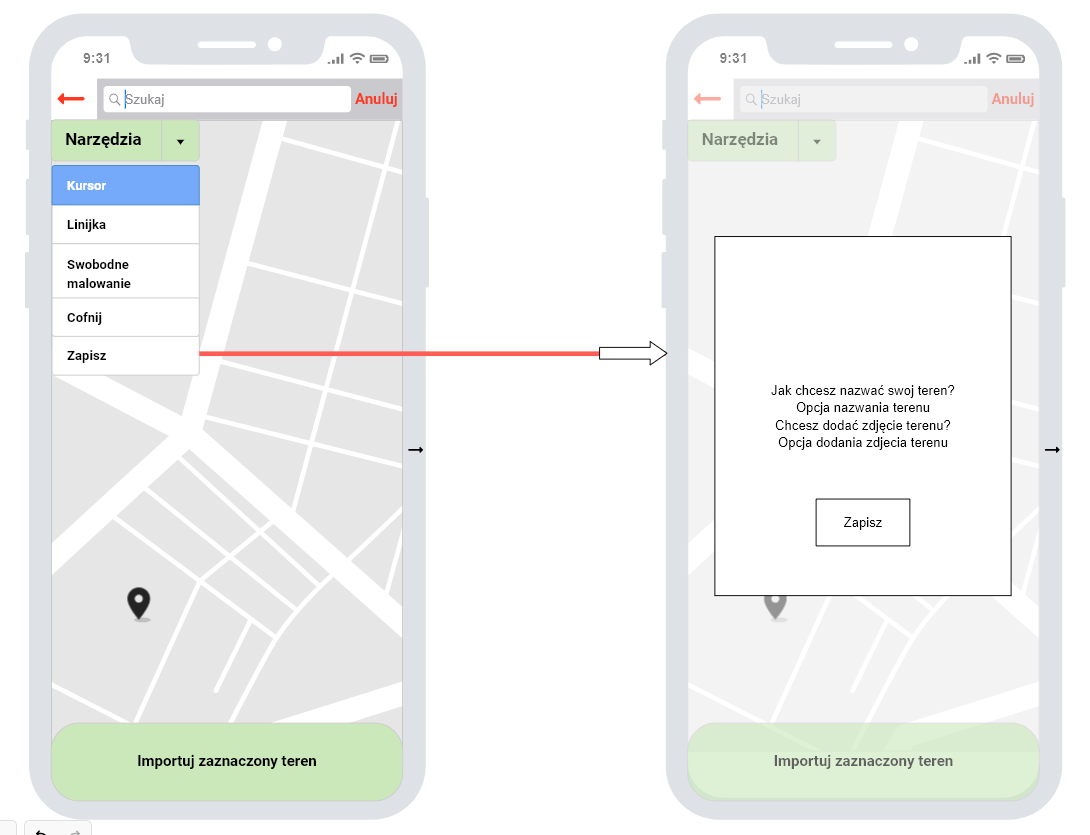
\includegraphics[width=15cm]{cipsko4.png}
  \end{figure}    